\begin{frame}
    \begin{center}
        \vspace{2.5cm}
        \normalsize
        \textbf{Игровые программы. Основы проектирования.} \\
        \vspace{2.0cm}
        \raggedleft\smallВыполнил:\\Голубев~А.~В., САПР-1.1п\\
        \vspace{2.0cm}
        \vspace{\fill}
        \centeringВолгоград \the\year
    \end{center}
\end{frame}

\begin{frame}
    Оглавление:
    \tableofcontents
\end{frame}

\section{Классификация компьютерных игр}
\begin{frame}
    \frametitle{Классификация компьютерных игр}
    Классификация компьютерный игр по жанрам:
    \begin{minipage}[t]{0.47\textwidth}
        \begin{itemize}
            \item Shooter
            \item Action
            \item Adventure
            \item Arcade
            \item Fighting
            \item FPS и TPS
            \item Hack and Slash
        \end{itemize}
    \end{minipage}
    \begin{minipage}[t]{0.47\textwidth}
        \begin{itemize}
            \item Interactive fiction
            \item Puzzle
            \item Rhythm game
            \item RPG
            \item RTS и TBS
            \item Simulator
            \item Traditional
        \end{itemize}
    \end{minipage}
\end{frame}

\section{Специализации разработчиков}
\begin{frame}
    \frametitle{Специализации разработчиков}
    В состав типичной современной команды разработчиков обычно входят представители разных 
    специализаций представленных ниже:
    \begin{figure}
        \begin{minipage}{0.47\textwidth}
            \begin{itemize}
                \item Графика
                \item Дизайн
                \item Звук
                \item Контроль качества
                \item Программирование
                \item Управление
            \end{itemize}
        \end{minipage}
        \begin{minipage}{0.5\textwidth}
            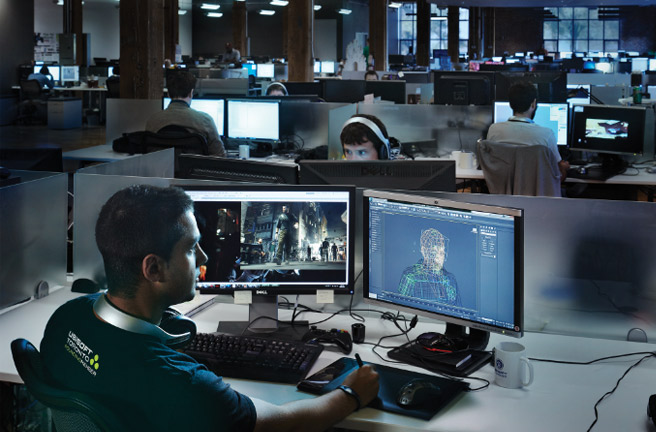
\includegraphics[width=1.0\textwidth]{ubisoft}
        \end{minipage}
    \end{figure}
\end{frame}

\section{Процесс разработки}
\begin{frame}
    \frametitle{Процесс разработки}
    Процесс разработки игры меняется в зависимости от компании и проекта. Однако разработка 
    коммерческой игры обычно включает следующие стадии:
    \begin{figure}
        \begin{minipage}{0.47\textwidth}
            \begin{itemize}
                \item Предпроизводственный процесс
                \item Производство
                \item Поддержка
            \end{itemize}
        \end{minipage}
        \begin{minipage}{0.5\textwidth}
            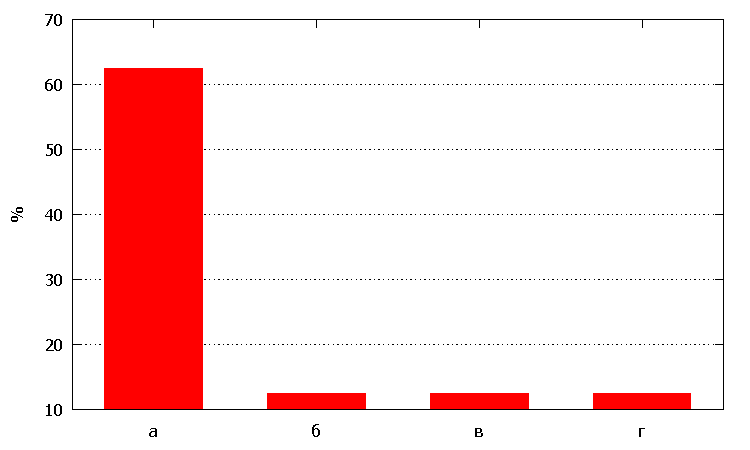
\includegraphics[width=1.0\textwidth]{work}
        \end{minipage}
    \end{figure}
\end{frame}

\begin{frame}
    \frametitle{Процесс разработки}
    \framesubtitle{Предпроизводственный процесс}
    Предпроизводственный процесс включает в себя следующие пункты:
    \begin{figure}
        \begin{minipage}{0.47\textwidth}
            \begin{itemize}
                \item Формирование идеи
                \item Определение жанра
                \item Создание геймплея
                \item Эскизный проект
                \item Документация проектировщика
            \end{itemize}
        \end{minipage}
        \begin{minipage}{0.5\textwidth1}
            
\includegraphics[width=1.0\textwidth]{idea}
        \end{minipage}
    \end{figure}
\end{frame}

\begin{frame}
    \frametitle{Процесс разработки}
    \framesubtitle{Производственный процесс}
    Производственный процесс состоит из работы над:
    \begin{itemize}
        \item Процесс разработки
        \begin{itemize}
            \item Программирование
            \item Графика
            \item Дизайн
            \item Эффекты
            \item Звук
        \end{itemize}
        \item Контроль качества
        \item Управление разработкой
    \end{itemize}
\end{frame}

\begin{frame}
    \frametitle{Процесс разработки}
    \framesubtitle{Процесс поддержки}
    Поддержка готового продукта состоит из:
    \begin{itemize}
        \item Исправление ошибок и выпуск патчей
        \item Расширение игровой функциональности
        \item Выпуск DLC
    \end{itemize}
\end{frame}

\section{Аутсорсинг}
\begin{frame}
    \frametitle{Аутсорсинг}
    Планы касательно аутсорсинга рассматривают на этапе подготовки производства; именно тогда 
    рассчитывают необходимые временные и финансовые затраты на работу, которая будет произведена вне 
    компании-разработчика.
    \begin{itemize}
        \item Модульные инструменты
        \item Музыкальные треки
        \item Актёрская озвучка
        \item Захват движений
    \end{itemize}
\end{frame}